%!TEX root = ../main.tex

\chapter{Bilder}

Bilder werden wie folgt eingefügt. Dabei sind verschiedene Arten möglich:

\begin{enumerate}
    \item Pfad inkl. Name
    \item Kurz-Unterschrift (erscheint später im Abbildungsverzeichnis)
    \item Unterschrift (erscheint später direkt unter dem Bild)
    \item label des Bildes; Format \textit{fig:label-text}
\end{enumerate}

Ein normales Bild einsetzen sieht so aus:

\begin{figure}[h]
    \centering
    \vspace{12pt}
    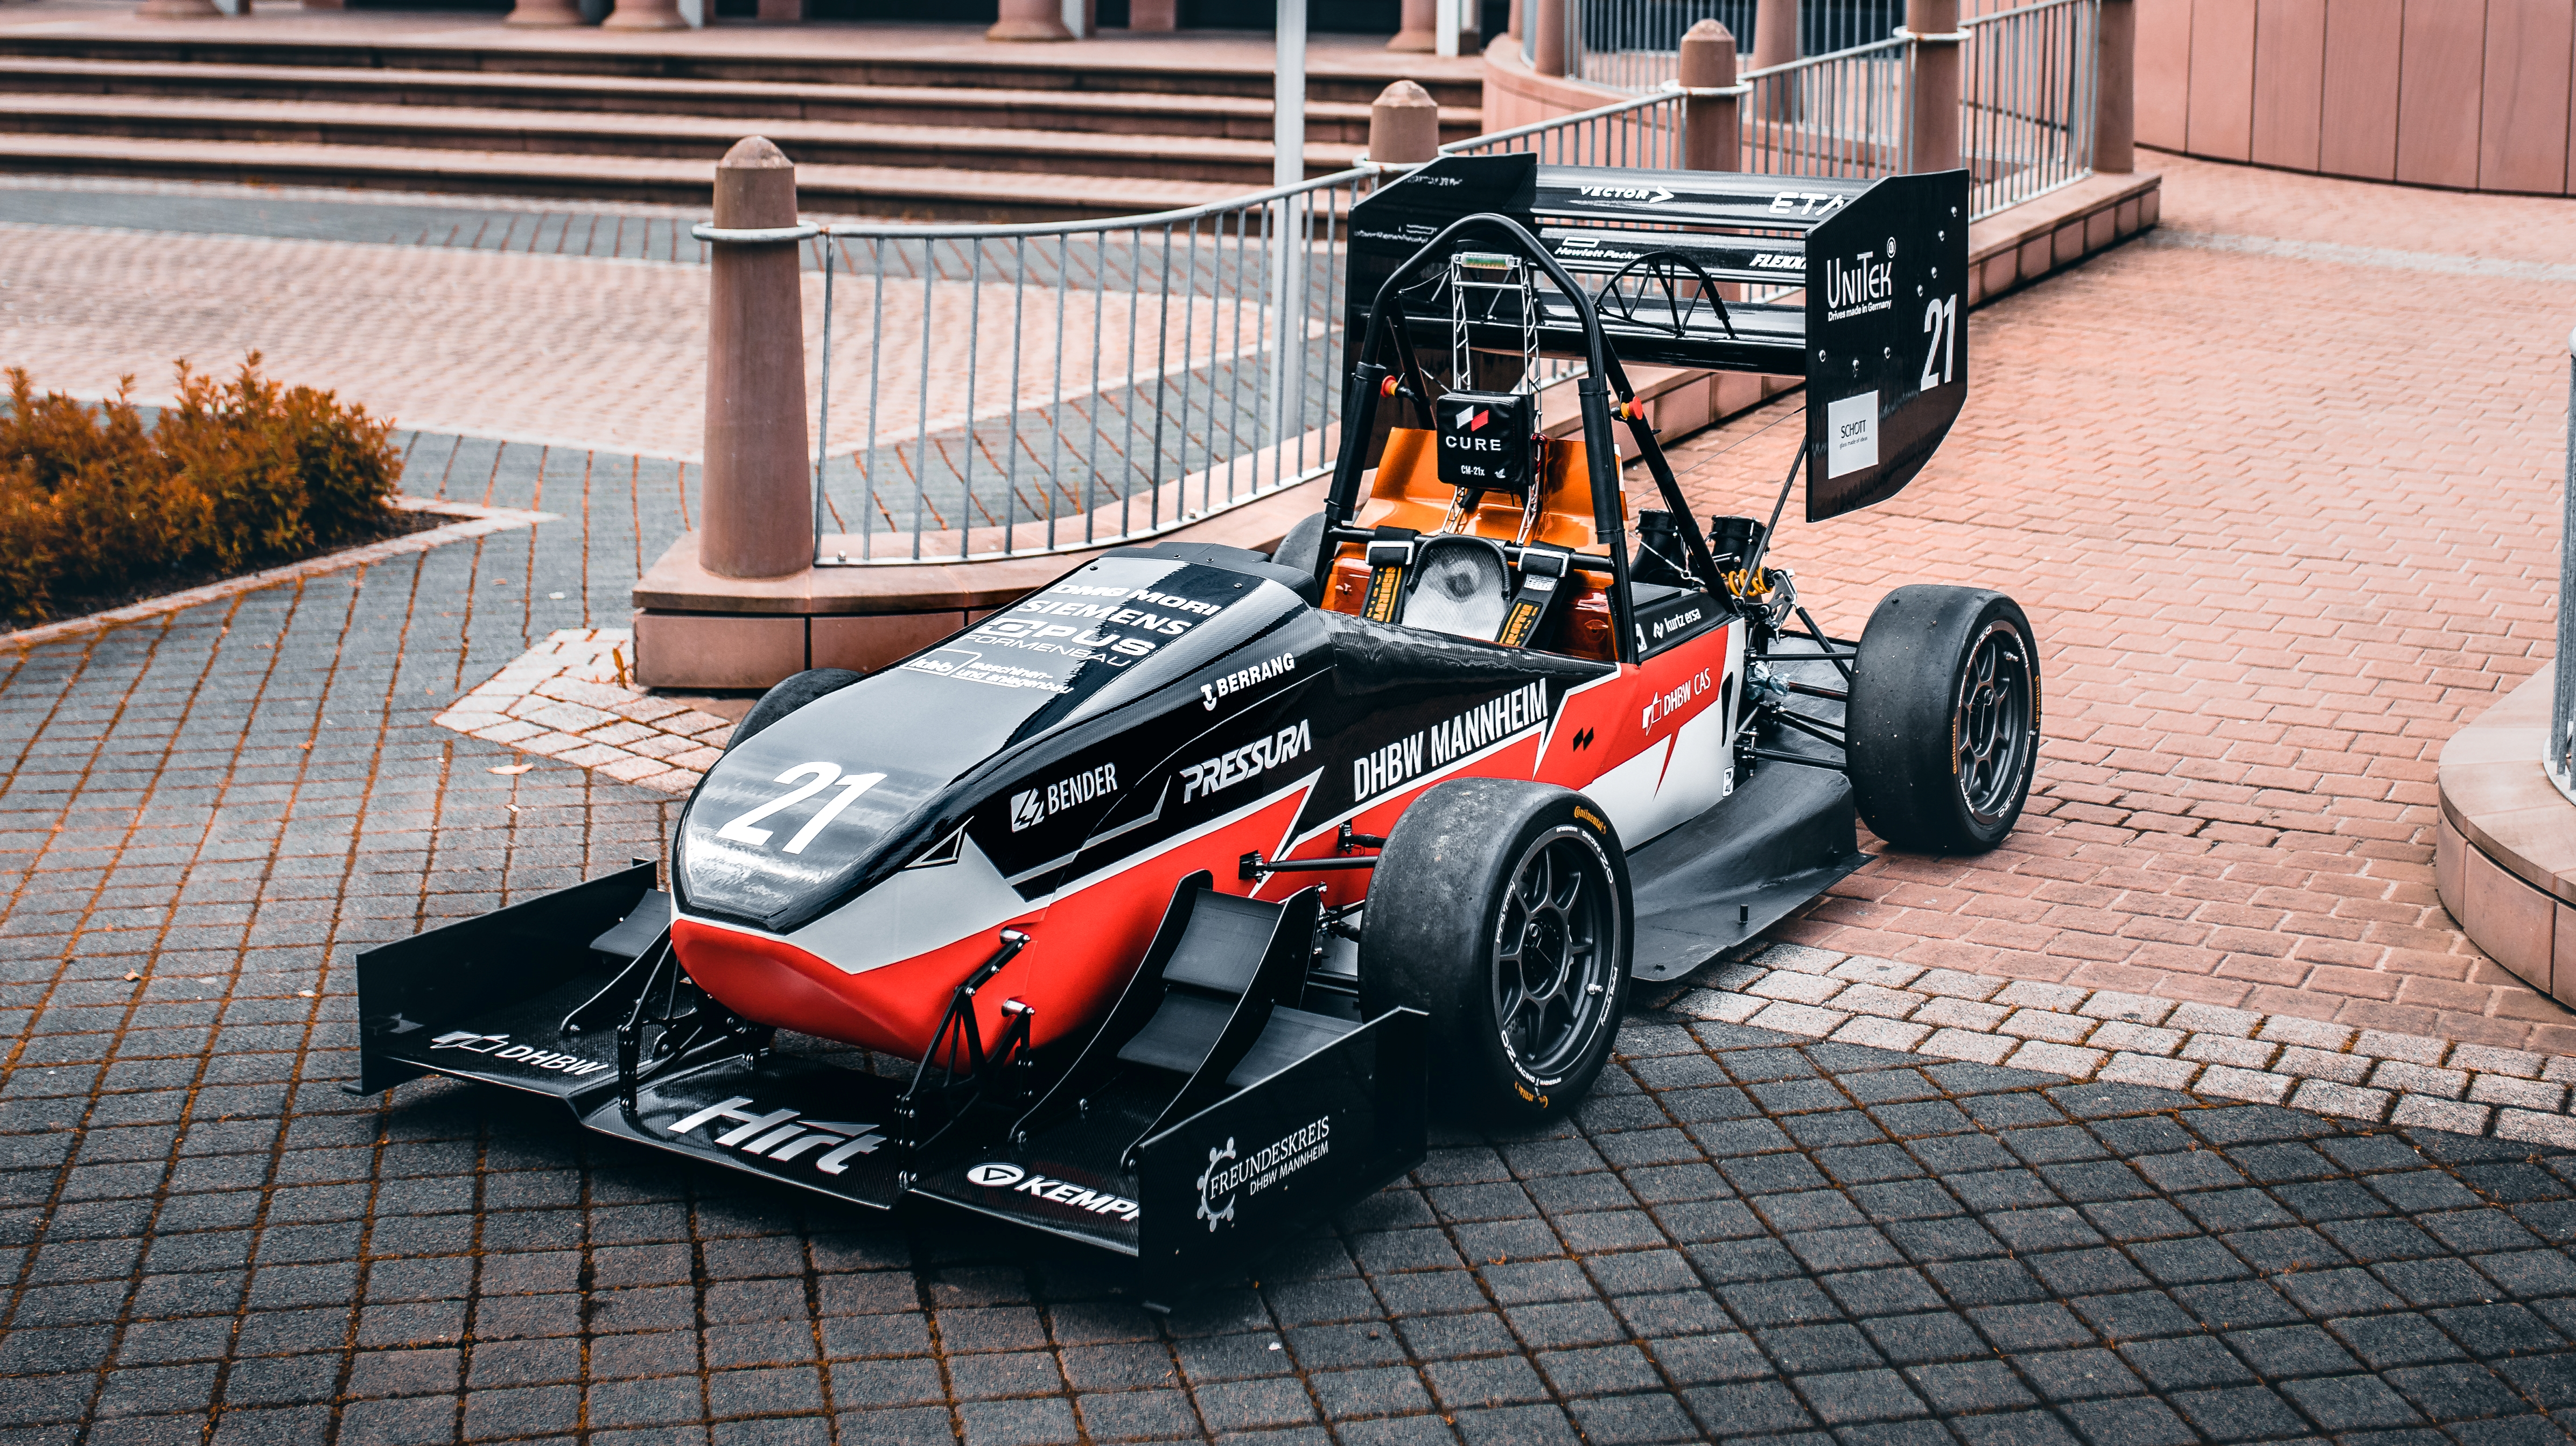
\includegraphics[width=0.7\textwidth]{images/EVA_Overview.jpg}
    \caption[Fahrzeug \glqq{}CM-21x\grqq{} ({\itshape EVA})]{Fahrzeug \glqq{}CM-21x\grqq{} ({\itshape EVA}) des Teams CURE in der Doppelsaison 19/21}
    \label{eva_overview}
\end{figure}

Zwei oder mehrere Bilder nebeneinander platzieren geht folgendermaßen:

\begin{figure}[H]
    \centering
    \begin{subfigure}[b]{.49\textwidth}
        \centering
        \includegraphics[width=.9\textwidth]{images/essential/firmenlogo.png}
        \vspace{4pt}
        \caption{}
        \label{fig:subfigure:a}
    \end{subfigure}
    \begin{subfigure}[b]{.49\textwidth}
        \centering
        \includegraphics[width=.9\textwidth]{images/essential/firmenlogo.png}
        \vspace{6pt}
        \caption{}
        \label{fig:subfigure:b}
    \end{subfigure}
    \caption{Zwei Bilder nebeneinander}
\end{figure}

Ein Bild kann aber auch mit Text umlaufend gesetzt werden:

\begin{wrapfigure}{r}{.7\textwidth}
    \centering
    \includegraphics[width=.6\textwidth]{images/essential/firmenlogo.png}
    \vspace{12pt}
    \caption{Overview of the proof of concept}
    \label{fig:overview}
\end{wrapfigure}
At first, an overview of the structure of the proof of concept is given in figure \ref{fig:overview}.
It is divided into two parts: \cite{Barg.2018} \\
Aliquam vehicula lectus elementum nulla finibus dignissim. Aliquam erat volutpat. Integer et dignissim leo. Suspendisse porta malesuada ante, malesuada ornare ex volutpat quis. Class aptent taciti sociosqu ad litora torquent per conubia nostra, per inceptos himenaeos. Nam enim neque, tristique ut mauris in, consectetur ultricies diam. Phasellus vulputate nibh at est placerat venenatis. Pellentesque maximus neque ut risus pretium rhoncus. Morbi tristique tristique nisl, eget molestie diam egestas a. Nulla posuere maximus dolor, sed tempus erat tincidunt sed. Praesent eget aliquam tellus. Vestibulum sed fringilla risus. Fusce egestas vestibulum fringilla.
    
Each part will be elaborated on subsequently.